\documentclass[12pt,final,twoside]{report}

\usepackage{thesis}

%%%%%%%%%%%%%%%%%%%%%%%%%%%%%%%%%%%%%%%%%%%%%%%%%%%%%%%%%%%%%
% Document:

\begin{document}

\pagenumbering{Roman}                   % Roman pagenumbering for lists and meta pages
\renewcommand{\headheight}{14.5pt}      % Size of headings

\thispagestyle{empty}
\fancyhead[LO,RE]{}                     % Define the header style for the meta pages

%%%%%%%%%%%%%%%%%%%%%%%%%%%%
% Cover sheet

\begin{titlepage}
%---Possibility 1:
    \begin{flushleft}
        
\includegraphics[width=85mm]{uhhLogoL.pdf}\\
    \end{flushleft}
%---Possibility 2:
%\includegraphics*[width=0.09\textwidth]{uhhIconR_}
%\parbox[c]{10cm}{
%    \begin{center}
%    Universit"at Hamburg --- MIN-Fakult"at\\
%    \trfachgruppe
%    \end{center}
%    }\hfill
%\includegraphics*[width=0.09\textwidth]{infIcon_}
%\vspace{0.2cm}
%---
    \rule{\textwidth}{0.4pt}
        \newline
        \vspace{2.0cm}
        \begin{center}
          \LARGE \textbf{\trtitle}
        \end{center}
    \vspace{2.0cm}
    \begin{center}
      \textbf{\trtype}\\
      %am Fachgebiet \trfach\\
      im Arbeitsbereich \trfach\\
      \trgutachterA\medskip\\
      Department Informatik\\
      MIN-Fakult\"at\\
      Universit\"at Hamburg \\[0.5cm]
      vorgelegt von \\
      \textbf{\trauthortitle\href{mailto:\tremail}{\trauthor}}\\
      am\\
      \trdate
    \end{center}
    \vspace{1cm}
    \begin{center}
    \begin{tabular}{ll}
    Gutachter: & \trgutachterA \\
                   & \trgutachterB \\
    %Betreuung: & \trbetreuung \\    	% Adviser are not allowed to demand getting credited, but are happy getting credited by the students initiative
    \end{tabular}
    \end{center}
    \vfill
    \begin{tabular}{l}
    \trauthor \\
    Matrikelnummer:  \trmatrikelnummer \\
    \trstrasse \\
    \trort
    \end{tabular}
    \newline
    \rule{\textwidth}{0.4pt}
    \newpage 
\end{titlepage}

    %backsite of cover sheet is empty!
\thispagestyle{empty}
\hspace{1cm}
\newpage

%%%%%%%%%%%%%%%%%%%%%%%%%%%%
% Abstract:
\chapter*{Abstract}
\thispagestyle{empty}
%\fancyhead[LE,RO]{\it Abstract}
%\addcontentsline{toc}{chapter}{\numberline{}Abstract}
Comparing to traditional visual object recognition, multimodal object recognition is advantageous in that different modalities provide complementary information. This work aims to implement a system for object recognition given videos of interactions with objects and investigate different modality fusion methods.

The bag-of-words model with SIFT descriptors and the MFCC are used as visual and audio features. The system classify objects by computing the probability with learned hidden Markov models. The system incorporates two different fusion methods: feature level fusion and decision level fusion. The former method learns a joint probability distributions with one HMM, while the latter method learns two separate probability distribution with two HMMs and combine them under the conditional independence assumption.

Experiments based on a dataset of 33 different household objects are carried out to evaluate the performance of these two fusion methods as well as single modality approaches. The result shows that both fusion methods improved the performance over single modality methods, while these two methods are mostly comparable. 

%\fancyhead[LE,RO]{\it Abstract}

\cleardoublepage

%%%%%%%%%%%%%%%%%%%%%%%%%%%%
% Lists:
\setcounter{tocdepth}{1}               % depth of the table of contents (for BSc and MSc Thesis 1 is recommented)
\fancyhead[LE,RO]{\it Contents}
\tableofcontents
\cleardoublepage
% List of Figures and List of tables are optional. -> Not needed in most theses.
\fancyhead[LE,RO]{\it List of Figures}
\listoffigures
\cleardoublepage
\fancyhead[LE,RO]{\it List of Tables}
\listoftables
\cleardoublepage
%\lstlistoflistings
%\cleardoublepage

\fancyhead[LE]{\it \leftmark}           % Define the header style for the text pages
\fancyhead[RO]{\it \rightmark}          % Define the header style for the text pages
\fancyhead[LO,RE]{}                     % Define the header style for the text pages

%%%%%%%%%%%%%%%%%%%%%%%%%%%%
% The content will be included here:
\pagenumbering{arabic}

\chapter{Introduction}
Considering how humans recognize objects, we use not only our vision, but also perceptions of other modalities, such as auditory, haptic and olfactory perceptions. These extra perceptions provide complementary information. This idea of multimodal object recognition can also be applied to robotic systems.

Traditional object recognition systems, which are exclusively based on visual information, are limited in several ways. They are sensitive to a number of image transformations such as view point change, occlusion and lighting variation. There are also cases, where the visual information alone is not sufficient to distinguish an object. For example, a paper cup might have the same appearance as a ceramic cup, and it is difficult to distinguish them only with vision. However, if we strike or touch them, we can get auditory or haptic feedback, from which it is possible to tell the difference.

Recent advances in robotics make it possible for robots to interact with objects and hence acquire multimodal information for object recognition. The study of how to use multimodal information for object recognition has become an important research topic.

\section{Related Work}

Nakamura et al.~\cite{nakamura_multimodal_2007} proposed an unsupervised object categorization method for robots based on visual, audio and haptic information. In their experiment, a robot hand was used to grasp and shake the objects. They first extracted the SIFT descriptors for vision, MFCCs for audio and pressure data for haptic information. Then, the bag-of-words models were used to represent all the input information. For categorization, they used a multimodal pLSA model, which is extended from the pLSA model for visual object categorization~\cite{sivic_discovering_2005}.

Sinapov and Stoytchev~\cite{sinapov_object_2011} proposed a behavior-grounded relational learning method for multimodal object recognition. They used an upper-torso humanoid robot to interact with the objects and collect proprioceptive and auditory information. The proprioceptive and audio information were further quantized individually with self-organizing map (SOM) to get sequences of SOM state indices. The similarity between two different sequence was be calculated with Needleman-Wunch alignment algorithm~\cite{needleman_general_1970}. With the similarity, they get the relational features, which are the average similarities to a known object sets. Consequently, they applied discriminative methods, like support vector machine, k-nearest neighbors and Decision Tree, for learning the object category.

Although research in multimodal object categorization/recognition has been carried out, there is no such object recognition system that uses visual and audio information. The study by Nakamura et al. used visual and audio information. However, their work focused on unsupervised categorization of unlabeled data. The study by Sinapov and Stoytchev was aimed for object recognition, but they avoid to use visual information, which is essential for understanding the object.

\section{Objective}
The specific objective of this study is to build an object recognition system based on visual and audio information from videos of interactions with objects. To achieve such goal, three basic questions need to be answered:
\begin{enumerate}
  \item What kind of features does the system use to represent the visual and audio information?
  \item How does the system make classification?
  \item How does the system combine multimodal information? 
\end{enumerate}

 The type of feature plays a critical role in the whole system. Good features make the learning trivial and bad features make the learning impossible.
 The system should incorporate a learning method that fits the data.
Good way to fuse multimodal information should favor reliable signals and avoid influence of noisy signals.

It is important to note that, concerning object recognition, there are two types of tasks been studied: specific object recognition and object category recognition~\cite{grauman_visual_2011}. The specific object recognition is the task of recognizing a particular object. \Cref{fig:specific} shows an example of specific object recognition. For training, the system is shown with a set of objects. For testing, one of the objects is presented, and the system need to tell which object it is.

Unlike the specific case, generic category recognition deal with classifying an instance to a category. \Cref{fig:generic} shows an example of generic category recognition. For training, the system is given a set of objects, some of which belongs to a category (positive instances) and some of which does not (negative instances). For testing, the system need to tell whether an unseen object belongs to this category or not. The generic category recognition is more challenging since the objects belongs to the same category vary in appearance.

\begin{figure}[t]
  \centering
  \begin{subfigure}[b]{.9\textwidth}
    \includegraphics[width=\textwidth]{specific.tikz}
    \caption{Specific object recognition.}
    \label{fig:specific}
  \end{subfigure}

  ~

  \begin{subfigure}[b]{.9\textwidth}
    \includegraphics[width=\textwidth]{generic.tikz}
    \caption{Generic category recognition.}
    \label{fig:generic}
  \end{subfigure}

  \caption{Two types of object recognition task.}
\end{figure}

\section{Thesis Outline}
\Cref{ch:visual} will present the bag-of-words model with SIFT descriptors, which is suitable use as the visual feature for our application.
\Cref{ch:audio} will present how to extract MFCCs as the audio feature.  
In \Cref{ch:hmm}, we will introduce the theories of hidden Markov models.  
In \Cref{ch:bimodal}, we will describe the design of our bimodal object recognition system. Two modality fusion methods will be discussed.  
\Cref{ch:experiment} will address how experiments are carried out and show the experiment results.  
Finally in \Cref{ch:conclusion}, our findings from the experiment will be discussed and suggested future work will be addressed.

\cleardoublepage

\chapter{Visual Features}
\label{ch:visual}

Visual object recognition has been extensively studied in the recent decade. Vision is very essential for both humans and artificial agents to recognize an object, since the appearance of the object provides us with the most direct and informational features. Numerous features have been proposed for visual object recognition and they have been used in a variety of applications.

In this chapter, we will present the state-of-the-art representation of object images using local features and the bag-of-words model, which is based on local features.

\section{Local Features}
Thinking of representing an object in an image, one method is extracting patterns that describe the whole picture, such as using the intensities of pixels. These methods are the global image representations. However, since the structures of most object appearances are very complex and the images are also subject to lighting variations, scaling, rotations, translations as well as occlusions, such global image representations can hardly generate robust results. 

In contrast to global representations, the local feature representation uses features of a local patches or regions to describe the image. These representations are designed to be invariant to a range of image transformations, such as scaling, rotation, translation and affine deformation. The development of such local features in the past decade has made it possible to implement robust and efficient object recognition applications.

A local feature extraction consists of the following two steps: 
\begin{description}
  \item[Keypoint detection] Detect a set of points of interest (i.e. keypoints) and the region around it, in a scale- or affine-invariant manner. Examples of keypoints detection methods include the Laplacian-of-Gaussian (LoG) detector~\cite{lindeberg_feature_1998}, the difference-of-Gaussian (DoG) detector~\cite{lowe_object_1999}, Harris affine detector~\cite{mikolajczyk_scale_2004} and maximally stable external regions (MSER)~\cite{matas_robust_2004}. 
  \item[Feature description] For each keypoint, compute its descriptor, which is a feature vector that describe the local region. Examples of feature description methods include the scale invariant feature transform (SIFT) and ``speed-up'' robust features (SURF)~\cite{bay_speeded-up_2008}.
\end{description}

Once descriptors are extracted, the similarity between images can be computed via comparing the local features they have. This yields a direct application for specific object recognition.

In the following section, we will introduce the DoG detector and the SIFT descriptor, as these methods are used in our system.

\subsection{The difference-of-Gaussian Detector}
The keypoint detection should be in a way that it can be repeated with different images of the same object. Therefore, the detectors are required to be scale or affine invariant. The difference-of-Gaussian (DoG) detector is an instance of scale invariant detectors.

Given an image $I(x)$, the DoG detector finds the position $x$ and the scale $\sigma$ that maximize (locally) the difference-of-Gaussian:
\begin{equation}
  D(x,\sigma) = (G(x,k\sigma) - G(x,\sigma)) * I(x)
\end{equation}
where $G(x,\sigma)$ is the Gaussian convolution mask, $k$ is a constant and $*$ is convolution. An efficient way to calculating the DoG is first smoothing (convoluting) the image with Gaussian mask at different scale, and then subtracting the results with the adjacent scales. Local maxima are located in several layers of DoG filtered images (each at different scales), such that $D(x,\sigma)$ is larger than the eight neighbors in same layer and the nine neighbors on each of the adjacent layers.

After the local maxima are found, an additional filtering step is added, in order to remove the points on edges. This is accomplished by evaluating the Hessian matrix at the points.

At the end, the selected points with the regions surrounding them (typically, $r = 3\sigma$) are extracted for further processing.

\subsection{The SIFT Descriptor}
The scale invariant feature transform (SIFT) descriptor is one of the state-of-the-art features that are used for visual object recognition. SIFT was originally published in papers by Lowe~\cite{lowe_object_1999,lowe_distinctive_2004}. 
Although in the original papers, the SIFT descriptor is designed with the DoG detector, it can also be combined with other detection methods~\cite{mikolajczyk_performance_2005}.

Once keypoints are located, the feature description of the keypoints should be in the way that it is invariant to many image transformations. What the keypoints detectors, such as DoG detector, has already achieved is scale and translation invariance. In addition to that, the SIFT descriptor provides features that are invariant to rotation and illumination variation.

The SIFT descriptor describes a keypoint as histograms of gradient orientations. Specifically, it is computed via the following steps:
\begin{enumerate}
  \item Normalize the size and orientation of the region around the keypoint according the scale, which is the result of scale invariant detector, and the dominant orientation.
  \item The region is divided to a $16 \times 16$ regular grid. For each location, the gradient orientation is computed.
  \item These locations are again divide into a $4 \times 4$ regular grid. For each cell, the gradient orientation histogram with 8 orientation bins is computed according to the gradient magnitudes applied with a Gaussian window.
  \item Combining the $16$ histograms will result in a $16 \times 8 = 128$ dimensional vector. Normalize this vector and the result is the SIFT descriptor.
\end{enumerate}

The rotation invariance is achieved by the selecting the dominant orientation in the first step and the illumination invariance is achieved by the normalization in the last step.

\begin{figure}[t]
  \centering
  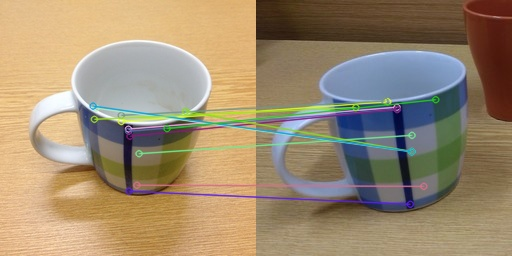
\includegraphics[width=.7\linewidth]{mug2m}
  \caption{Example of feature matching with SIFT descriptors.}
  \label{fig:match}
\end{figure}

An example of feature matching with SIFT descriptors is shown in \cref{fig:match}. Two images of an object is taken from different view points and under different lighting condition. The identical keypoints from the two images are detected with SIFT descriptors.

\section{The Bag-of-Words Model}
While specific object recognition can be solved as matching of local features, the local feature representation cannot be directly applied to object category recognition. Local features are adequate in characterizing an exact part of a particular object. However, different objects in the same category are not identical in appearance. Thus, in this case, a valid representations should capture the common characteristics of different instances in the same class. One of the solution is the bag-of-words model~\cite{csurka_visual_2004}.

The bag-of-words model has been originally used in nature language processing. The idea is considering a document as a multiset consisting of words, that is counting the number of occurrences and disregarding the order of the words. Therefore, a document can be represented as a histogram of distinctive words. The bag-of-words model has been successfully applied to a number of nature language processing and information retrieval tasks, such as text classification.

\begin{figure}[t]
  \centering
  \includegraphics[width=.8\textwidth]{bow.tikz}
  \caption{Example of bag-of-words model.}
  \label{fig:bow}
\end{figure}


Analogous to natural text, an image, which contains a collection of keypoints (or local feature descriptors), can also regarded as an document. And, this is the idea of the bag-of-words model for computer vision. In this case, the model is also referred as bag of visual words, bag of feature or bag of keypoints. 

However, there is an essential difference between a word and a local feature descriptor, which is that a word is a nominal value while a descriptor is a real vector. Thus, a vector quantization step is carried out to map a descriptor to a visual ``word''. In most of the applications, the descriptors are quantized by matching to the nearest neighbor in a vocabulary, which is constructed in advance by clustering, such as k-means. Another benefit from quantization is that the different but similar descriptors are put into the same class. Therefore, the representation is more robust to variations between objects in the same category.

Similar to that in nature language processing, images represented by bag-of-words model can be used for further learning. These applications includes supervised classification using support vector machine or na\"ive Bayes~\cite{csurka_visual_2004} and unsupervised categorization using probabilistic latent semantic analysis or latent Dirichlet allocation~\cite{sivic_discovering_2005}.

\section{Summary}
In this chapter, we have presented the local features and the bag-of-words model for visual object recognition. The key points include:
\begin{itemize}
  \item The local feature representation is one of the state-of-art technique for computer vision. The representation is computed via keypoint detection and feature description. The results are a number of descriptors of the points of interest in the image. 
  \item The DoG detector is invariant to scaling.
  \item The SIFT descriptors are invariant to rotation and illumination variation.
  \item The Bag-of-words model, which is based on local features, is a more general representation of a image. 
\end{itemize}

\cleardoublepage
\chapter{Audio Features}
\label{ch:audio}
Audio signal processing has been one of the most important fields of digital signal processing. Many different audio features have been proposed to represent the audio signal. As for any system, how the data is represented affects the performance of the system dramatically. And, so is for our system. In terms of good audio features, we want to find features such that, similar sounds that human perceive also appear similar (closer) in the feature space and the number of dimensions of the feature space should be small so that it can be applied to the subsequent learning algorithms. In other words, the feature should be simple and corresponds to human perception.

Although audio features for object recognition have not been systematically studied, there has been extensive studies on audio features for speech recognition. The mel-frequency cepstrum coefficients (MFCCs) is one of the most commonly used audio features in speech recognition. Therefore, we choose MFCCs as the audio feature in our system.

In this chapter, we will present the basics about preprocessing of audio signal, namely short time Fourier transform, and the properties of the MFCCs.

\section{Short Time Fourier Transform}
The raw audio data are represented as the altitudes of the pressure changing over time, i.e. time-domain signal. However, the time-domain signal does not contain direct information of how the signal sounds like. Thus, it is difficult be analyzed. By applying the Fourier transform, we can change the signal to frequency domain. In the frequency domain, further analysis of the signal can be applied.

The power spectrum, i.e. the squared magnitude of the Fourier transform, shows how the energy is distributed in different frequency bin, but it does not show how the signal varies over time. That means it cannot specify the local information at a certain time. The solution to this problem is the short time Fourier transform (STFT), which transform the signal to the time-frequency domain.

The idea of STFT is that by using a sliding window, the signal at a short time is taken, and then applying the Fourier transform. More specifically, the STFT is defined as follows:
\begin{equation}
  X(n, k) = \sum_{m = -\infty}^{\infty} x[m]w[m-n]e^{-j \frac{2\pi k}{N} m}
\end{equation}
where $x$ is the signal, $w$ is the window function, $n$ is the index of time, $k$ is the index of frequency bin, and $N$ is the number of frequency bins. 

Common window functions include the Hann window:
\begin{equation} w(n) = 0.5 (1 - \cos(\frac{2\pi n}{N-1})) \end{equation}
and the Hamming window:
\begin{equation} w(n) = \alpha - \beta \cos(\frac{2\pi n}{N-1}) \end{equation}
where $\alpha = 0.54, \beta = 1 - \alpha = 0.46$ and $N$ is the window size.
Since, most applications in practice use the fast Fourier transform to compute the STFT, the window size is selected to be an exponential of 2.

The squared magnitude of the STFT yields the spectrogram:
\[ \text{Spectrogram}(n, k) = \left|X(n,k)\right|^2 \]
From the spectrogram we can clearly visualize the different frequency components of a sound and its variation over time.

Note that because the time-domain signal is real, at any time, the result of the DFT has the following properties:
\begin{itemize}
  \item $X(n,0)$ and $X[n, \frac{N}{2}]$ are real;
  \item $X(n,k) = X^*(n,N-k), k \neq 0, \frac{N}{2}$, here $^*$ is the complex conjugate.
\end{itemize}

Therefore, only the first half (index from $0$ to $\frac{N}{2}$) of the DFT contains information, while the other half is redundant. From theories of Fourier analysis, we know that the $k$th frequency bin represents the component at frequency $\frac{kf_s}{N}$, with $f_s$ being the sampling rate. The component with the highest frequency is the bin with index $\frac{N}{2}$ and its frequency is $\frac{N}{2} \times \frac{f_s}{N} = \frac{f_s}{2}$. This is, in fact, the Nyquist frequency.

\begin{figure}[t]
  \centering
  \begin{subfigure}[b]{.8\textwidth}
    \includegraphics[width=\textwidth]{spec1024}
    \caption{$N=1024$}
    \label{fig:spec1024}
  \end{subfigure}

  \begin{subfigure}[b]{.8\textwidth}
    \includegraphics[width=\textwidth]{spec256}
    \caption{$N=256$}
    \label{fig:spec256}
  \end{subfigure}

  \begin{subfigure}[b]{.8\textwidth}
    \includegraphics[width=\textwidth]{spec64}
    \caption{$N=64$}
    \label{fig:spec64}
  \end{subfigure}

  \caption[Spectrograms with different window sizes]{Spectrograms of audio ``Hello World'' with different window sizes ($N$). (a) When the window size is $1024$, the spectrogram shows high frequency resolution, yet low time resolution.
    (b) When the window size is $256$, the spectrogram shows moderate frequency resolution and time resolution.
    (c) When the window size is $64$, the spectrogram shows low frequency resolution and high time resolution.
  The STFT is calculated with a shift size of half window size. }
  \label{fig:spec}
\end{figure}

One shortcoming for STFT is that the frequency resolution and time resolution is mutually limited. This limit is known as the Gabor limit. The difference of two consecutive frequency bin is $\frac{f_s}{N}$. And, one STFT is a DFT of a neighborhood of $N$ samples, i.e. $N \times \frac{1}{f_s}$ time interval. That means the time resolution is $\frac{N}{f_s}$. Therefore, the product of the two resolutions, $\frac{f_s}{N} \times \frac{N}{f_s} = 1$, is constant. 

Selecting the windows size involves trade-off between the frequency resolution and time resolution. With large window size, we can have good frequency resolution, while it can be difficult to catch the change in a short time. Vice versa, with a small windows size, we can have high time resolution. However, the frequency resolution would be low. \Cref{fig:spec} illustrates these difference.

\section{Mel-frequency Cepstrum Coefficients}
Despite the fact that the STFT gives information how the audio signal distributed at different frequencies over time, the frequency (i.e. pitch) is not the only characteristic human hear from a sound. Thus, the STFT itself is not a desired feature. However, the spectral information derived from the STFT can be further analyzed, which results in several spectral features. Among these features, the mel-frequency cepstrum coefficients (MFCCs) are commonly used for speech recognition.
The MFCCs are the coefficients of a cepstrum with frequency bands on the mel scale.

The mel scale is the scale of frequencies based on human perception of the distance in pitches. Classic study shows that human perceive the pitches in a non-linear scale~\cite{stevens_scale_1937}, which if usually formulated as~\cite{oshaughnessy_speech_1987}
\begin{equation}
  \text{mel} = 1127 \log (1 + \frac{f}{700})
\end{equation}

A cepstrum is a ``spectrum'' of log spectrum. The term cepstrum is a result of reversing the first four letters in spectrum. The idea of using a ``spectrum'' of log spectrum was prompted by detecting echo in signals~\cite{oppenheim_frequency_2004}. Consider a signal with a simple echo
\begin{equation}
  x(t) = s(t) + \alpha s(t - \tau),
\end{equation}
where $s(t)$ is the original signal and $\tau$ is the echo delay, the spectrum of the signal is
\begin{equation}
  \left| X(f) \right|^2 = \left| S(f) \right|^2 (1 + \alpha^2 + 2 \alpha \cos(2 \pi f \tau)),
\end{equation}
and the log spectrum is
\begin{equation}
  C(f) = \log \left| X(f) \right|^2 = \log \left| S(f) \right|^2 + \log (1 + \alpha^2 + 2 \alpha \cos(2 \pi f \tau)).
\end{equation}
Consider $C(f)$ as a signal of $f$, it has an additive periodic component due to the present of the $\cos$ term and its ``fundamental frequency'' is the echo delay $\tau$. Therefore, taking the Fourier transform of $C(f)$, the ``spectrum'' shows a peak at the ``fundamental frequency''. 

The computation of MFCCs consists of the following steps:
\begin{enumerate}
  \item Compute the STFT of the original time-domain signal.
  \item For each time frame, map the spectrum onto mel scale, using triangular overlapping windows.
  \item Take the log of spectrum based on mel scale.
  \item Take the discrete cosine transform of the log spectrum.
\end{enumerate}

\section{Summary}
In this chapter, we have presented some of the features for audio processing. The key points include:
\begin{itemize}
  \item The STFT is one of the basic preprocessing of audio signal, which transform time-domain signals to the time-frequency domain.
  \item The MFCC is a audio feature that gives interpretation of sounds that is similar to human perception. It also captures information such as echo in the signal.
\end{itemize}

\cleardoublepage
\chapter{Theories of Hidden Markov Model}
\label{ch:hmm}
The hidden Markov models (HMM) are statistical models for time series data, which have been well-known and widely used by researchers~\cite{rabiner_tutorial_1989, rabiner_fundamentals_1993}. Theories of HMM are initially published by Baum and his colleagues~\cite{baum_statistical_1966, baum_maximization_1970}. They have been successfully applied to a number of research fields, including speech processing~\cite{baker_dragon_1975, rabiner_fundamentals_1993}, image processing~\cite{chen_off-line_1994}, gesture recognition~\cite{mitra_gesture_2007}, bioinformatics~\cite{koski_hidden_2001}, finance~\cite{bhar_hidden_2004}, etc.

In this chapter, we will first introduce the formal definition of the HMM and then present the algorithms for evaluating probability and estimating the model parameters.

\section{Definition of HMM} \label{sec:hmm}
A hidden Markov model describes a probability distribution of a stationary discrete-time stochastic process under certain assumptions. These assumptions include that there is an unobserved or hidden state associated with every observation at each time and the states transition meets the Markov property (i.e. Markov assumption). More precisely, for one observed sequence, $\mathbf{x} = x_1 x_2 \dots x_T$, and its associated state sequence, $\mathbf{q} = q_1 q_2 \dots q_T$, the following properties hold:

\begin{enumerate}
  \item The conditional distribution of present observation (at a certain time $t$) depends only upon the present hidden state:
    \begin{equation}
      P(x_t|q_1, \dots, q_t, x_1, \dots, x_{t-1},x_{t+1},\dots,x_T) = P(x_t|q_t), \quad t \in \mathbb{N} 
      \label{eq:ob_prob}
    \end{equation}
  \item (Markov property) The conditional probability distribution of future hidden state of the process depends only upon the present state:
    \begin{equation}
      P(q_{t+1}|q_1, \dots, q_t, x_1, \dots, x_t) = P(q_{t+1}|q_t),\quad t \in \mathbb{N}
      \label{eq:markov_prop}
    \end{equation}
\end{enumerate}

\begin{figure}[t]
  \centering
  \includegraphics{hmm.tikz}
  \caption[HMM as a Bayesian network.]{HMM as a Bayesian network. The directed edges indicate conditional dependencies. Each state variable is only conditional dependent of its previous state and each observation is only conditional dependent of the state at that time.}
  \label{fig:hmm}
\end{figure}

These conditional dependencies can be shown as a Bayesian network by unfolding the variables over time (see \cref{fig:hmm}).

Here, the observation can be on a discrete space ($x_t \in \{v_1, v_2, \dots, v_K\}$) or a continuous space ($x_t \in \mathbb{R}^d$) and the state space is discrete ($q_t \in \{1, 2, \dots, N\}$, with $N$ being the number of states). Since our system is exclusively used on continuous data, for simplicity, we will only consider the continuous observation space. Gaussian mixture models (GMM) are usually used to describe such observation probability distribution. In this case, the model is called HMM-GMM.

Given the aforementioned assumptions, one HMM can be specified with the following parameters:
\[ \lambda = (A, B, \pi) \]
such that
\begin{itemize}
  \item $A$ is the transition probability, $A = \{a_{ij}\}$, in which 
    \[ a_{ij} = P(q_{t+1} = j | q_t = i), \quad i,j \in \{1, \dots, N\} \]
  \item $B$ is the observation probability distribution, $B = \{b_j(x)\}$, in which
    \[ b_j(x) = P(x_t = x | q_t = j), \quad i,j \in \{1, \dots, N\} \]
  \item $\pi$ is the initial state distribution, $\pi = \{\pi_j\}$, in which
    \[ \pi_j = P(q_1 = j), \quad i,j \in \{1, \dots, N\} \]
\end{itemize}

As for HMM-GMM, each $b_j(x)$, more specifically, is a probability density function (pdf) of a GMM, namely
\[ b_j(x) = \sum_{k=1}^M c_{jk} \mathcal{N}(x, \mu_{jk}, \Sigma_{jk}) \]
where $c_{jk}$ is the mixture weight (coefficient), $\mu_{jk}$ is the mean and $\Sigma_{jk}$ is the covariance matrix, each of the $k$-th component in state $j$ and $\mathcal{N}$ is the pdf of the Gaussian distribution. 

With the formal definition of HMM, there are still three problems of interest to be solved, in order to use HMM for real-world applications. These problems are:
\begin{enumerate}
  \item Given a model $\lambda=(A, B, \pi)$, and an observation sequence $\mathbf{x} = (x_1 x_2 \dots x_T)$, what is the probability of the model generating such sequence, namely $P(\mathbf{x}|\lambda)$?
  \item Given a model $\lambda$, and an observation sequence $\mathbf{x}$, what is the most likely hidden state sequence $\mathbf{q} = (q_1 q_2 \dots q_t)$, namely $\argmax_{\mathbf{q}}P(\mathbf{x}|\mathbf{q},\lambda)$?
  \item Given an observation sequence $\mathbf{x}$ (or a set of observations $\{\mathbf{x}^{(i)}\}$), how do we estimate the parameters that maximize $P(\mathbf{x}|\lambda)$ (or $\prod_{i} P(\mathbf{x}^{(i)}|\lambda) $)?
\end{enumerate}

In the following section, we will show that the first and third problem can be solved using the forward/backward procedure and the Baum-Welch algorithm, respectively. The second problem can be solved using the Viterbi algorithm~\cite{forney_viterbi_1973}. However, the second problem is not related to our system, so it will not be addressed.

\section{Probability Evaluation}
Given a model $\lambda=(A, B, \pi)$, and an observation sequence $\mathbf{x} = (x_1 x_2 \dots x_T)$, we wish to calculate the probability, $P(\mathbf{x}|\lambda)$. A na\"ive solution to this is enumerating all possible state sequences and applying law of total probability, that is
\begin{equation}
  P(\mathbf{x}|\lambda) = \sum_{\text{all } \mathbf{q}} P(\mathbf{x}|\mathbf{q},\lambda) P(\mathbf{q}|\lambda) .
\end{equation}

For a fixed state sequence $\mathbf{q} = (q_1 q_2 \dots q_T)$, we can derive that
\begin{align}
  P(\mathbf{x}|\mathbf{q},\lambda) &= P(x_1|q_1,\lambda) P(x_2|q_1,q_2,x_1,\lambda) \dots P(x_T|q_1,\dots,q_T,x_1,\dots,x_{T-1},\lambda) \notag\\
  &= P(x_1|q_1, \lambda) P(x_1|q_1, \lambda) \dots P(x_T|q_T, \lambda) \notag\\
  &= b_{q_1}(x_1) b_{q_2}(x_2) \dots b_{q_T}(x_T)
\end{align}
and its probability is
\begin{align}
  P(\mathbf{q}|\lambda) &= P(q_1|\lambda) P(q_2|q_1,\lambda) P(q_3|q_1,q_2,\lambda) \dots P(q_T|q_1,\dots,q_{T-1},\lambda) \notag\\
  &= P(q_1|\lambda) P(q_2|q_1,\lambda) P(q_3|q_2,\lambda) \dots P(q_T|q_{T-1},\lambda)  \notag\\
  &= \pi_{q_1} a_{q_1q_2} \dots a_{q_{T-1}q_T} .
\end{align}
Thus we get 
\begin{equation}
  P(\mathbf{x}|\lambda) = \sum_{q_1,q_2,\dots,q_T} \pi_{q_1} b_{q_1}(x_1) a_{q_1q_2} b_{q_2}(x_2) \dots a_{q_{T-1}q_T} b_{a_T}(x_T) .
  \label{eq:prob_brute}
\end{equation}

This is a direct solution, however, the number of possible state sequences is too large, which is $N^T$. Thus, the time efficiency would be $\Theta(T N^T)$ using big theta notation. That makes it impossible to calculate when $T$ is large, which is often the case. In the following part, we will present the forward procedure and the backward procedure, which are more efficient.

\subsection{The Forward Procedure}
One of the efficient solution is using the forward procedure. Consider the forward variable, $\alpha_t(i)$, which is the joint probability or the first $t$ observations and the state at time $t$, or defined as
\begin{equation}
  \alpha_t(i) = P(x_1,\dots,x_t,q_t=i|\lambda) 
\end{equation}
it has the following properties:
\begin{enumerate}
  \item At initial time,
    \begin{equation}
      \alpha_1(i) = P(x_1,q_1=i|\lambda) = \pi_i b_i(x_1), \qquad i \in \{1,\dots,N\} .
    \end{equation}
  \item The forward variable at $t \geq 2$ can be calculated via considering it is transitioned from all the possible previous states:
    \begin{align}
      \alpha_{t+1}(j) &= P(x_1,\dots,x_{t+1},q_{t+1}=j|\lambda) \notag\\
      &= \sum_{i=1}^{N} P(x_1,\dots,x_{t+1},q_t=i,q_{t+1}=j|\lambda) \notag\\
      &= \sum_{i=1}^{N} P(x_1,\dots,x_t,q_t=i|\lambda) P(q_{t+1}=j|q_t=i,\lambda) P(x_{t+1}|q_{t+1}=j,\lambda) \notag\\
      &= \left[ \sum_{i=1}^{N} a_{ij} \alpha_t(i) \right] b_j(x_{t+1}), \qquad t \in \{1,\dots,T - 1\}, j \in \{1,\dots,N\} .
    \end{align}
  \item Take the sum of all the forward variables at time $t = T$, we get the desired calculation of the probability,
    \begin{equation}
      P(\mathbf{x}|\lambda) = \sum_{i=1}^N P(\mathbf{x},q_T=i|\lambda) = \sum_{i=1}^N \alpha_T(i) .
    \end{equation}
\end{enumerate}

By using the three properties, we can iteratively calculate all the $N$ forward variables from time $1$ to $T$. The time efficiency of the forward procedure is $\Theta(TN^2)$, which much faster than using the na\"ive solution (\cref{eq:prob_brute}).

\subsection{The Backward Procedure}
The backward procedure is an alternative solution to calculating the probability. Similar to the forward procedure, the backward procedure use the same idea of iterative calculation of variables based on previous steps, while the direction of iteration is backward, namely from $T$ to $1$. The backward variable is defined as
\begin{equation}
  \beta_t(i) = P(x_{t+1},\dots,x_T|q_t=i,\lambda) .
\end{equation}

The following properties hold:
\begin{enumerate}
  \item At time $t = T$,
    \begin{equation}
      \beta_T(i) = 1, \qquad i \in \{1,\dots,N\} .
    \end{equation}
  \item The backward variable at $t \leq T - 1$ can be calculate inductively:
    \begin{align}
      \beta_i(t) &= \sum_{j=1}^{N} P(x_{t+1},\dots,x_T,q_{t+1}=j|q_t=i,\lambda) \notag\\
      &= \sum_{j=1}^{N} P(q_{t+1}=j|q_t=i,\lambda) P(x_{t+1}|q_{t+1}=j,\lambda) P(x_{t+2},\dots,x_T|q_{t+1}=j,\lambda) \notag\\
      &= \sum_{j=1}^{N} a_{ij} b_j(x_{t+1}) \beta_{t+1}(j) , \qquad t \in \{1,\dots,T - 1\}, j \in \{1,\dots,N\} .
    \end{align}
  \item The probability is
    \begin{equation}
      P(\mathbf{x}|\lambda) = \sum_{i=1}^N P(\mathbf{x}|q_1=i,\lambda) p(q_1=i|\lambda) = \sum_{i=1}^N \beta_1(i) \pi_i .
    \end{equation}
\end{enumerate}

Same as the forward procedure, the time efficiency of the backward procedure is $\Theta(TN^2)$.

\section{Parameter Estimation}
Parameter estimation of a statistical model is the adjustment of the parameters such that the model can best match the observed or empirical data. It plays a crucial role in systems. As for HMM, we are interested in knowing what are the parameters that maximize the probability of the observation (i.e. maximum likelihood estimates):
\begin{equation}
  \lambda^* = \argmax_{\lambda} P(\mathbf{x}|\lambda) .
\end{equation}

Unlike simple models, such as Gaussian distributions, the parameters of which can be calculated directly, HMM depends on unobserved latent variables (i.e. hidden states), which make it difficult to estimate. One general solution for parameter estimation of models with latent variables is the expectation-maximization (EM) algorithm. The application of the EM algorithm for HMM is known as the Baum-Welch algorithm. We will shows these two algorithms in the following part.

\subsection{Expectation-maximization Algorithm}
The expectation-maximization algorithm is a method for finding the maximum likelihood estimates (MLE) of parameters of models with latent variables~\cite{dempster_maximum_1977}. Its idea is reestimating parameters via an expectation step (E-step) and a maximization step (M-step), in which the reestimated parameters have greater likelihood, and repeating such procedure until the likelihood reaches a maximum.

More specifically, consider observed data $\mathbf{x}$, unobserved data (i.e. latent variables) $\mathbf{z}$ and a set of parameters $\lambda$, the likelihood function is
\begin{equation}
  L(\lambda;\mathbf{x}) = P(\mathbf{x}|\lambda) = \sum_{\mathbf{z}} P(\mathbf{x},\mathbf{z}|\lambda) .
\end{equation}
The goal is maximizing the likelihood function:
\begin{equation}
  \lambda^* = \argmax_\lambda L(\lambda;\mathbf{x}).
\end{equation}

We introduce a function $Q(\lambda|\lambda')$, which is the conditional expectation of the log likelihood function with respect to the conditional distribution of $\mathbf{z}$ given $\mathbf{x}$ and $\lambda'$:
\begin{equation}
  Q(\lambda|\lambda') = \text{E}_{\mathbf{z}|\mathbf{x},\lambda'} \log P(\mathbf{x},\mathbf{z}|\lambda) .
\end{equation}

A procedure of parameters reestimation consists of the following two steps:
\begin{description}
  \item[E-Step] Compute $Q(\lambda|\lambda^{(p)})$;
  \item[M-Step] Choose $\lambda^{(p+1)}$ to be the value of $\lambda$ that maximize $Q(\lambda|\lambda^{(p)})$.
\end{description}

After each procedure it is assured that $L(\lambda^{(p+1)};\mathbf{x}) \geq L(\lambda^{(p)};\mathbf{x})$. Therefore, if we start from an initial estimate $\lambda^{(0)}$ and iteratively compute $\lambda^{(1)},\lambda^{(2)},\lambda^{(3)},\dots$, we will get a sequence of estimates, which converges to a local maximum.

The increase of likelihood function can be proved as follows: for any $\mathbf{z}$, we have
\begin{equation}
  \log P(\mathbf{x}|\lambda) = \log P(\mathbf{x},\mathbf{z}|\lambda) - \log P(\mathbf{z}|\mathbf{x},\lambda). 
\end{equation}
For both sides, if we multiply $P(\mathbf{z}|\mathbf{x},\lambda')$ and sum over all $\mathbf{z}$, we get
\begin{align}
  \sum_{\mathbf{z}} P(\mathbf{z}|\mathbf{x},\lambda') \log P(\mathbf{x}|\lambda) 
  &= \sum_{\mathbf{z}} P(\mathbf{z}|\mathbf{x},\lambda') \log P(\mathbf{x},\mathbf{z}|\lambda)
  - \sum_{\mathbf{z}} P(\mathbf{z}|\mathbf{x},\lambda') \log P(\mathbf{z}|\mathbf{x},\lambda) \notag\\
  \log P(\mathbf{x}|\lambda) &= Q(\lambda|\lambda') + H(\lambda|\lambda')
  \label{eq:loglph}.
\end{align}
Here, $H(\lambda|\lambda')$ is defined as
\begin{equation}
  H(\lambda|\lambda') = - \sum_{\mathbf{z}} P(\mathbf{z}|\mathbf{x},\lambda') \log P(\mathbf{z}|\mathbf{x},\lambda)
\end{equation}
From Gibbs' inequality we know that, for any $\lambda$ and $\lambda'$
\begin{equation}
  H(\lambda|\lambda') \geq H(\lambda|\lambda),
\end{equation}
with equality if and only if $\lambda = \lambda'$. Therefore, together with \cref{eq:loglph},
\begin{align}
  \log P(\mathbf{x}|\lambda) - \log P(\mathbf{x}|\lambda') &= Q(\lambda|\lambda') - Q(\lambda'|\lambda') + H(\lambda|\lambda') -  H(\lambda|\lambda) \notag\\
  & \geq Q(\lambda|\lambda') - Q(\lambda'|\lambda')
\end{align}

Since $\lambda^{(p+1)}$ is a maximum of $Q(\lambda|\lambda^{(p)})$, $Q(\lambda^{(p+1)}|\lambda^{(p)}) - Q(\lambda^{(p)}|\lambda^{(p)}) \geq 0$. Therefore, $L(\lambda^{(p+1)};\mathbf{x}) \geq L(\lambda^{(p)};\mathbf{x})$.

It is important to note that although the EM algorithm converges to a maximum estimate, there is no guarantee that the estimate is a global maximum (thus not a MLE). The resulting estimate depends on the initial estimate. Therefore, additional heuristic methods should be chosen for application of the EM algorithm.

\subsection{Baum-Welch Algorithm}
We have shown that the EM algorithm can be used for parameter estimation for models with latent variables and HMMs are examples or such models. Thus, applying the EM algorithm to the HMM would result in a solution for the third problem we stated in \cref{sec:hmm}. This method is known as the Baum-Welch algorithm.

Before we proceed to derive the reestimation formulas, we first define variables $\gamma_t(i) = P(q_t=i|\mathbf{x},\lambda)$ and $\xi_t(i,j) = P(q_t=i,q_{t+1}=j|\mathbf{x},\lambda)$, which can be computed as follows:
\begin{align}
  \gamma_t(i) &= \frac{P(\mathbf{x},q_t=i|\lambda)}{P(\mathbf{x}|\lambda)} \notag\\
  &= \frac{\alpha_t(i)\beta_t(i)}{P(\mathbf{x}|\lambda)} ,
  \label{eq:hmmgamma}
\end{align}
and
\begin{align}
  \xi_t(i,j) &= \frac{P(\mathbf{x},q_t=i,q_{t+1}=j|\lambda)}{P(\mathbf{x}|\lambda)} \notag\\
  &=  \frac{\alpha_t(i)a_{ij}b_j(x_{t+1})\beta_{t+1}(j)}{P(\mathbf{x}|\lambda)} .
  \label{eq:hmmxi}
\end{align}

Now, we put the HMM into the frame of the EM algorithm.

\paragraph{E-step}
Consider parameters $\lambda=(A,B,\pi)$ and $\lambda'=(A',B',\pi')$ 
\footnote{We use `` $'$ '' to indicate parameters or variables from the previous estimate.}
, compute $Q(\lambda|\lambda')$:
\begin{align}
  Q(\lambda|\lambda') &= \sum_{\mathbf{q}} P(\mathbf{q}|\mathbf{x},\lambda') \log P(\mathbf{x},\mathbf{q}|\lambda) \notag\\
  &= \sum_{\mathbf{q}} \frac{P(\mathbf{x},\mathbf{q}|\lambda')}{P(\mathbf{x}|\lambda')} 
  (\log \pi_{q_1} + \sum_{t=1}^{T-1} \log a_{q_t q_{t+1}} + \sum_{t=1}^{T} \log b_{q_t}(x_t) ) \notag\\
  &= \frac{1}{P(\mathbf{x}|\lambda')} (Q_\pi(\pi|\lambda') + Q_A(A|\lambda') + Q_B(B|\lambda'))
  \label{eq:qhmmsep}
\end{align}
where
\begin{align}
  Q_\pi(\pi|\lambda') &= \sum_{\mathbf{q}} P(\mathbf{x},\mathbf{q}|\lambda') \log \pi_{q_1}  \notag\\
  &= \sum_{i=1}^{N} p(\mathbf{x},q_1=i|\lambda') \log \pi_{i} \notag\\
  &= \sum_{i=1}^{N} \gamma'_1(i) \log \pi_{i},
\end{align}
\begin{align}
  Q_A(A|\lambda') &= \sum_{\mathbf{q}} P(\mathbf{x},\mathbf{q}|\lambda') \sum_{t=1}^{T-1} \log a_{q_t q_{t+1}} \notag\\
  &= \sum_{i=1}^{N} \sum_{j=1}^{N} \sum_{t=1}^{T-1} P(\mathbf{x},q_t=i,q_{t+1}=j|\lambda') \log a_{ij} \notag\\
  &= \sum_{i=1}^{N} \sum_{j=1}^{N} (\sum_{t=1}^{T-1} \xi'_t(i, j)) \log a_{ij}
\end{align}
and
\begin{align}
  Q_B(B|\lambda') &= \sum_{\mathbf{q}} P(\mathbf{x},\mathbf{q}|\lambda') \sum_{t=1}^{T} \log b_{q_t}(x_t) \notag\\
  &= \sum_{i=1}^{N} \sum_{t=1}^{T} p(\mathbf{x},q_t=i|\lambda') \log b_{i}(x_t) \notag\\
  &= \sum_{i=1}^{N} \sum_{t=1}^{T} \gamma'_t(i) \log b_{i}(x_t) .
  \label{eq:qhmmb}
\end{align}

\paragraph{M-step}
For fixed $\mathbf{x}$ and $\lambda'$, to maximize $Q(\lambda|\lambda')$, we can see from \cref{eq:qhmmsep} that we only need to find parameters $\pi$, $A$ and $B$ that maximize $Q_\pi(\pi|\lambda')$, $Q_A(A|\lambda')$ and $Q_B(B|\lambda')$, individually.

In order to be a valid distribution, the parameters subjects to the following constraints
\begin{align}
  \sum_{i=1}^{N} \pi_i &= 1  \\
  \sum_{j=1}^{N} a_{ij} &= 1 , \qquad \forall i 
\end{align}
and $b_i(x)$ is a valid probability density function of a GMM.

From Gibb's inequality, we know that the maximum of 
\begin{equation}
  \sum_{i=1}^N w_i \log y_i
\end{equation}
subject to $\sum_{i=1}^N y_i = 1$, is attained when
\begin{equation}
  y_i = \frac{w_i}{\sum_{j=1}^N w_j} .
\end{equation} 
Therefore, the reestimation of $\pi$ and $A$ are
\begin{equation}
  \pi_i = \frac{\gamma'_1(i)}{\sum_{j=1}^N \gamma'_1(j)} = \gamma'_1(i)
  \label{eq:hmmpi}
\end{equation} 
and
\begin{equation}
  a_{ij} = \frac{\sum_{t=1}^{T-1} \xi'_t(i,j)}{\sum_{k=1}^N \sum_{t=1}^{T-1} \xi'_t(i,k)} = \frac{\sum_{t=1}^{T-1} \xi'_t(i,j)}{\sum_{t=1}^{T-1} \gamma'_t(i)}
  \label{eq:hmma}
\end{equation} 

For the parameters $B$, from \cref{eq:qhmmb}, we can see that is it similar to reestiamting the parameters in a GMM, except that the terms are weighted with the expected occurrences of that state, $\sum_{t=1}^{T} \gamma'_t(i)$. And the result is as follows~\cite{bilmes_gentle_1998}:
\begin{equation}
  c_{jk} = \frac{\sum_{t=1}^{T} \gamma'_t(j,k)}{\sum_{t=1}^{T} \sum_{l=1}^{M} \gamma'_t(j,l)},
  \label{eq:hmmc}
\end{equation}
\begin{equation}
  \mu_{jk} = \frac{\sum_{t=1}^{T} \gamma'_t(j,k) x_t}{\sum_{t=1}^{T} \gamma'_t(j,k)}
  \label{eq:hmmmu}
\end{equation}
and
\begin{equation}
  \Sigma_{jk} = \frac{\sum_{t=1}^{T} \gamma'_t(j,k) (x_t-\mu'_{jk})(x_t-\mu'_{jk})^T}{\sum_{t=1}^{T} \gamma'_t(j,k)}
  \label{eq:hmmsigma}
\end{equation}
where $\gamma'_t(j,k)$ is the probability of being state $j$ at time $t$ with the $k$-th mixture component (under the condition of the previous estimate $\lambda'$):
\begin{equation}
  \gamma'_t(j,k) = \gamma'_t(j) \frac{c'_{jk} \mathcal{N}(x_t,\mu_{jk},\Sigma_{jk})} {b_j(x_t)} . \label{eq:hmmgamma2}
\end{equation}

To summarize, the reestimation of HMM parameters consists of the following steps:
\begin{enumerate}
  \item Compute $\alpha'_t(i)$ and $\beta'_t(i)$ using the forward and backward procedures;
  \item Compute $\gamma'_t(i)$, $\xi'_t(i,j)$ as well as $\gamma'_t(j,k)$ using \cref{eq:hmmgamma,eq:hmmxi,eq:hmmgamma2};
  \item Compute the new parameters $\pi_i$, $a_{ij}$, $c_{jk}$, $\mu_{jk}$ and $\Sigma_{jk}$ using \cref{eq:hmmpi,eq:hmma,eq:hmmc,eq:hmmmu,eq:hmmsigma}.
\end{enumerate}
And, by repeating these steps, we can get an estimate of the parameters which attain a local maximum of the likelihood function.

\section{Summary}
In this chapter, we have presented the theories of hidden Markov models. The key points include:
\begin{itemize}
  \item HMMs are statistical models for time series data with latent variables (i.e. hidden states). The parameters include the initial state distribution, state transition probability and observation probability distribution.
  \item The probability of HMM can be computed using the forward or the backward procedure.
  \item The parameters of HMM can be estimated by the Baum-Welch algorithm, which is an application of the EM algorithm. However, the result is not assured to be a global optimum.
\end{itemize}

\cleardoublepage
\chapter{HMM for Bimodal Object Recognition}
\label{ch:bimodal}
So far we have introduced some methods for extracting visual and audio features as well as HMM, a statistical model for time series data. It is now sufficient to combine them together to build a system for visual-audio object recognition. This chapter describes and discusses the design of our system as well as the issues we meet upon implementing the system. 

Before proceeding to explain how the system is structured, it is necessary to mention that the goal is to build a system for recognizing objects from video recordings of interactions with the objects. To achieve this goal, the system should be designed in the way that:
\begin{itemize}
  \item The visual and audio representations can be effectively learned for category classification.
  \item The system utilized sequential relationship in signals, since an interaction is in essence perceived as images and sound which vary over time.
  \item A proper modality fusion method is selected in order to make vision and audio a good complement of each other.
\end{itemize}

This chapter is divided into three sections, each of which presents the system design relating to one of the goals above.

\section{Feature Extraction}
\subsection{Visual Processing Pipeline}
As mentioned in \cref{ch:visual}, the bag-of-words models with SIFT descriptors are powerful at representing the visual features of objects among the same category. And, the applications of bag-of-words models have achieved satisfying performance in visual object category recognition. Therefore, we use the bag-of-words models as the visual feature. The visual processing pipeline is shown in \cref{fig:vpipe}. 

\begin{figure}[t]
  \centering
  \includegraphics{vpipe.tikz}
  \caption{The visual processing pipeline.}
  \label{fig:vpipe}
\end{figure}

First, the image frames from the raw video are taken at frame rate of 5 frames per second. For each image frame, the keypoints are detected using the DoG keypoint detector. Then, the SIFT descriptors of all the keypoints are computed. All the descriptors are quantized using a codebook of visual descriptors, which is prepared in advance. After that, the number of occurrences of the visual ``words'' are counted and represented as a normalized histogram (i.e. the bag-of-words feature). Since the codebook used in the experiment contains 20 ``words'', the visual feature is a sequence of 20-dimensional vectors.

\subsection{Audio Processing Pipeline}
We choose the MFCCs as the audio feature, because the MFCCs have been commonly used in speech recognition, speaker recognition as well as music information retrieval applications. The audio processing pipeline is shown in \cref{fig:apipe}.

\begin{figure}[t]
  \centering
  \includegraphics{apipe.tikz}
  \caption{The audio processing pipeline.}
  \label{fig:apipe}
\end{figure}

The audio data are sampled at 8000 Hz. We first use shifting windows with window size of 1024 and shifting size of 1600 to get the audio frames, so that the rate of the audio frames is equal to that of the visual data. Then, we calculate the Mel-frequency cepstrum coefficients (MFCCs) with 32 filter banks. Among all the coefficients, from the second to the 17th are taken, resulting in a 16-dimensional vector. In this way, we get a sequence of MFCCs as the audio feature.

\section{Classification with HMM}
As our system requires a learning model which accounts for time series data, the HMM is a perfect choice in this case, for its effective application in speech recognition and gesture recognition. Besides, the HMM, which is a statistical model, allows us to estimate the probability, which can be used for further inference in modality fusion.

Classification using HMM required one model to be learned for each class $c$. The model for class $c$ is learned to describe the distribution of all the instances of this class, that is:
\begin{equation}
  \lambda^c = \argmax_{\lambda} \prod_{\mathbf{x} \in D^c} P(\mathbf{x}|\lambda^c)
\end{equation}
in which $D^c$ is the set of data instances of which the labels are $c$. The models are learned with the Baum-Welch algorithm. Then, when given a new instance of observation sequence, we can approximate the likelihood of a class with the learned model by
\begin{equation}
  P(\mathbf{x}|c) = P(\mathbf{x}|\lambda^c) .
\end{equation}

For specific category recognition, which is a multiclass classification problem, the prediction of a new instance is carried out by choosing the class with the maximum likelihood:
\begin{equation}
  f(\mathbf{x}) = \argmax_{c} P(\mathbf{x}|c) .
\end{equation}

For generic category recognition, the classification is carried out individually for each category. Thus, predicting whether an instance belongs to a certain category is a binary classification problem. The classification is based on comparing the posterior probability to a given threshold $\theta$:
\begin{equation}
  \label{eq:classif}
  f(\mathbf{x}) = 
  \left\{ \begin{array}{l l} +1, & \quad P(c=+1|\mathbf{x}) > \theta; \\ -1, & \quad \text{otherwise.}
  \end{array} \right.
\end{equation}

From Bayesian theory, the posterior probability of a class given the observation is
\begin{equation} \label{eq:posterior}
  P(c|\mathbf{x}) = \frac{P(\mathbf{x}|c)P(c)}{\sum_{c \in \{-1,+1\}} P(\mathbf{x}|c)P(c)}
\end{equation}
in which $P(c)$ is the prior probability of the class.

Considering the fact that randomly selecting objects as data set is not likely to be the same as randomly drawing a sample in a real world, the prior probability is hard to estimate. However, if we assume that the prior probabilities are equal, we still can have the same decision by varying the threshold. We will later evaluate the performance of a classifier using area under the receiver operating characteristic curve and such evaluation method is not affected by the threshold. Therefore, by assuming equal prior probabilities, \cref{eq:posterior} can be rewrite as 
\begin{equation}
  \label{eq:postsimp}
  P(c|\mathbf{x}) = \frac{P(\mathbf{x}|c)}{\sum_{c \in \{-1,+1\}} P(\mathbf{x}|c)} .
\end{equation}

\subsection{Model Selection}
An important issue about HMM is selecting the model size and the observation distribution, i.e. the number states, the number of components for each state and the type of covariance matrix. The choice of models can have a dramatic impact on the result.

For the number of states and the number of components, the larger the numbers are the more complex the model is. And the covariance matrix can be either a full matrix or a diagonal matrix. The diagonal matrix assumes the feature coefficients are not correlated, thus is simpler than full matrix.

\begin{table}[t]
  \caption{Comparison of simple and complex models.}
  \label{tab:model}
  \centering
  \begin{tabular}{p{.42\textwidth}p{.42\textwidth}}
    \toprule
    \multicolumn{1}{c}{\bfseries Simple Models} & \multicolumn{1}{c}{\bfseries Complex Models} \\ \midrule
    Smaller hypothesis space. & Larger hypothesis space. \\
    Easy to learn. & Hard to learn. \\
    Underfitting. & Overfitting. \\
    \bottomrule
  \end{tabular}
\end{table}

In general, complex models have larger hypothesis space, which also means more predictive power. However, since the Baum-Welch algorithm does not guarantee global optimum, more complex models are more prone to local optima. Furthermore, it could also result in overfitting if the training set is not large enough. The comparison of simple and complex models are listed in \cref{tab:model}.

Making decision for the model choice should follow the principle of Occam's razor. Depending on different data, the best choice is the simplest model that can fit the data.

\subsection{Implementation Issues}
Several implementation issues are addressed in the following part.

\subsubsection{Underflow and overflow}

When probabilities accumulate through the data sequence, the values can be significantly larger or smaller than $1$. Such values exceed the precision range of machines. To avoid such underflow and overflow problems, the computation is perform with the logarithmic values of each variable. 

\subsubsection{Insufficient training data}

As previously described in the Baum-Welch algorithm, the reestimation procedure requires a calculation of state probabilities based on a present estimation. Such state probabilities can be zero especially when the training set is insufficient. When a probability of a state is non-zero only with one or a few observations, it is impossible to estimate the covariance matrix. One way to tackle this issue is to set a minimal value along the diagonal of the covariance matrix. 

\subsubsection{Parallelization}

From our experience, the training process of the HMM parameters can take very long time. Our system incorporates parallel computation with OpenMP. The parallelization increases the speed up to 8 times of the original on a computer with an 8-core CPU.

\section{Methods for Multimodal Fusion}
Having discussed how to extract feature vectors and how to make decision based on it, the final part of system design addresses the question of how multimodal signals are fused. The way to fuse the visual and audio information is essential to the object recognition system, that good method makes use of both modalities and avoid noises from unreliable signal.

Multimodal fusion may be classified according to the level of fusion into feature level fusion, decision level fusion and hybrid fusion~\cite{atrey_multimodal_2010}. The feature level fusion or early fusion is the approach of combining the multimodal features before they are sent as input of a learning model. The decision level fusion or late fusion approach, on the other hand, analyzes each modality independently and then combines the individual decisions to a final result. The hybrid fusion is a combination of these two approaches.

The system incorporates two different designs regarding the fusion method: one with feature level fusion and the other with decision level fusion. Such methods will be presented in the remaining of this section. The performance of these two methods will be further discussed with experimental results in later chapters.

To ground our discussion, consider the problem of binary classification using HMM with visual and audio features. The observation is a combination of visual and audio features, $\mathbf{x} = (\mathbf{v}, \mathbf{a})$. To make a decision using \cref{eq:classif,eq:postsimp}, we need the to know the joint likelihood $P(\mathbf{v},\mathbf{a}|c)$.

\subsection{Feature Level Fusion}
\begin{figure}[t]
  \centering
  \includegraphics{featuref.tikz}
  \caption[Block diagram of the feature level fusion approach.]{Block diagram of the feature level fusion approach. Features of different modalities are first combined at the feature fusion module and then the joint probability is computed directly with the HMM which is learned with the combined feature.}
  \label{fig:featuref}
\end{figure}

A direct approach is simply learn the HMM with the concatenated features, therefore the joint likelihood can be approximated with 
\begin{equation}
  P(\mathbf{v},\mathbf{a}|c) = P(\mathbf{v},\mathbf{a}|\lambda_{va}^c)
\end{equation}
in which $\lambda_{va}^c$ are the estimated bimodal HMM parameters. This is an approach of feature level fusion. A block diagram of such approach is shown in \cref{fig:featuref}.

The advantage of feature level fusion is that it utilizes the correlation between modalities. Theoretically, if the HMM are properly chosen and well trained, the feature level fusion approach can yields optimal estimation of the joint likelihood. Learning both modalities at the same time increases the hypothesis space and also increases the difficulty of estimating the optimal parameters of the HMM.

\subsection{Decision Level Fusion}
\begin{figure}[t]
  \centering
  \includegraphics{decisionf.tikz}
  \caption[Block diagram of the decision level fusion approach.]{Block diagram of the decision level fusion approach. Likelihood of different modalities are first computed individually and then combined at the decision level under the conditional independence assumption.}
  \label{fig:decisionf}
\end{figure}

An alternative approach is learning separate HMMs and combine the likelihood at decision level. If we assume the features of different modalities are conditionally independent given the class, the joint likelihood can be computed as
\begin{equation}
  P(\mathbf{v},\mathbf{a}|c) = P(\mathbf{v}|c) P(\mathbf{a}|c) = P(\mathbf{v}|\lambda_v^c) P(\mathbf{a}|\lambda_a^c)
\end{equation}
in which $\lambda_{v}^c$ and $\lambda_{a}^c$ are the estimated HMM parameters for visual and audio features, respectively. A block diagram of such approach is shown in \cref{fig:decisionf}.

Rather than learning a complex HMM model, the decision level fusion approach learns two simple models. Therefore it is more likely to get a optimal estimation of the HMM parameters. However, the fusion is based on the assumption of conditional independence, which usually does not hold in reality. In this case, the joint likelihood estimation will be biased.

\section{Summary}
In this chapter, we have presented the design of a visual-audio object recognition system based on HMMs. The key points include:
\begin{itemize}
  \item The system uses bag-of-words model with SIFT descriptors as the visual feature and the Mel-frequency cepstrum coefficients as the audio feature.
  \item The system uses HMM to estimate probabilities. For specific object recognition, instances are classified by selecting the class with maximum likelihood. For generic category recognition, classification is carried out by comparing the posterior probability with a threshold. The model selection plays a crucial role to the system.
  \item The system incorporates two types of multimodal fusion methods. The feature level fusion method is to learn HMM with concatenated features and directly estimate the joint likelihood. The decision level fusion methods is to learn two HMMs for individual modalities and compute the joint likelihood with the conditional independence assumption. Such two methods will be compared in the experiment.
\end{itemize}

\cleardoublepage
\chapter{Experiment and Results}
\label{ch:experiment}
Experiments based on a visual-audio object dataset were carried out to evaluate different object recognition methods. The methods include feature fusion, decision fusion, visual only and audio only approaches. This chapter describes the experiment and the results.

\section{Dataset}
The dataset consists of videos of interactions with 33 different objects. The objects include household objects such as boxes, mugs, bowls and bottles. The materials of the objects range from ceramic to glass, paper, wood, metal and plastic. Some of the containers also have content inside.

The videos were taken from a webcam at a resolution of $640 \times 480$ pixels and frame rate of 10 frames per second. The sound was recorded from the microphone on the webcam at 16000 Hz. When recording, the object was place in the center of the view and take up a dominant part of the image. There was a few objects in the background.

Three different interactions, including \emph{striking}, \emph{pushing} and \emph{shaking}, were performed by the experimenter. Some of the interaction produced sound, while the others did not. Each combination of object and interaction are recorded multiple times from different view points.

Each object is given a set of labels indicating whether this object belongs to a category. Six categories are studied in the experiment, including \emph{mugs}, \emph{bottles}, \emph{plastic objects}, \emph{metal objects}, \emph{fragile objects} and \emph{containers with content}.  
A full list of objects with their categories can be found in \cref{app:dataset}. 

\section{Evaluation Criteria}
The performances of each method are evaluated with two different criteria for the two different tasks. 

\subsection{Evaluation of Specific Object Recognition}
For the specific object recognition task, the accuracy of each method is calculated with 5-fold cross validation. The accuracy (ACC) is the percentage of correctly classified instances, namely 
\[ \text{ACC} =  \frac{\text{\# correctly classified}}{\text{\# total}} . \]
For all methods, the HMM parameters are learned with two states, six mixture components for each states and diagonal covariance matrix.

\subsection{Evaluation of Generic Category Recognition}
For the generic category recognition task, we evaluate the classification performance with object-based validation. Each time the video instances of one object is separated from the whole dataset to be the testing data and the rest are used for training. Therefore, all the testing objects are unseen objects, which are not in the training set. The HMM parameters are learned with various number of states and mixture components. For each method, the best setting is selected to represent the result of the method.

In the case of generic category recognition, instead of accuracy we used the area under the receiver operating characteristic curve as the criterion. The accuracy does not comprehensively indicate the performance of a binary classifier. It is because there can be cases where more than 90 percents of the instances are negative and a trivial classifier which always predict negative would result in a rather high accuracy.

\begin{figure}[t]
  \centering
  \includegraphics[width=.5\textwidth]{roc.tikz}
  \caption[Example of a ROC curve.]{Example of a ROC curve. The curve is created by plotting the TPR against the FPR by varying the threshold. The dashed line shows the ROC curve of a random classifier. The green line at the upper left shows a ROC curve of a perfect classifier. The ROC curve of a normal classifier is expected to have a shape of the blue curve in the figure.}
  \label{fig:roc}
\end{figure}

Since the classification (\cref{eq:classif}) is based on a discrimination threshold, it is possible use the receiver operating characteristic (ROC) curve to evaluate the classification result. The ROC curve is generated by plotting the true positive rate (TPR) against the false positive rate (FPR) by shifting the threshold from $0$ to $1$ (\cref{fig:roc}). The TPR, also known as recall rate or sensitivity, is the percentage of conditionally positive instances being predicted to be positive by the classifier:
\[ \text{TPR} =  \frac{\text{\# true positive}}{\text{\# conditional positive}} . \]
The FPR, also known as fall-out rate, is the percentage of conditionally negative instances being predicted to be positive by the classifier:
\[ \text{FPR} =  \frac{\text{\# false positive}}{\text{\# conditional negative}} . \]

The area under the ROC curve (AUC) can indicate the performance of a binary classifier. An AUC of a classifier is expected to be between $0.5$ and $1.0$, with larger value indicating better performance. The AUC of a random classifier is $0.5$ and that of a perfect classifier is $1.0$.

\section{Results}
\subsection{Specific Object Recognition Results}
The accuracy of each method for the specific object recognition task is shown in \cref{tab:spec}. The performance of both feature fusion and decision fusion methods are better than the visual only and audio only methods. The improvement is about $10\%$. These two fusion methods are only slightly different in performance.

\begin{table}
  \caption{Results of specific object recognition.}
  \label{tab:spec}
  \centering
  \begin{tabular}[h!]{lc}
    \toprule
    \multicolumn{1}{c}{Method} & Accuracy \\ \midrule
    Feature Fusion & \textbf{95.8\%} \\
    Decision Fusion  & 95.7\% \\
    Visual Only & 86.7\% \\
    Audio Only & 83.6\% \\
    \bottomrule
  \end{tabular}
\end{table}

\subsection{Generic Category Recognition Results}
The results of generic category recognition is shown in \cref{tab:cateory} and \cref{fig:catroc}. For the recognition of mugs (\cref{fig:rocmug}), the decision fusion method has the best performance, followed closely by the visual only method and feature fusion method. For the recognition of bottles and plastic objects (\cref{fig:rocbottle,fig:rocplastic}), both fusion methods are better than the unimodal methods. For the recognition of metal objects (\cref{fig:rocmetal}), the visual only method is the best and the fusion methods are slightly worse. For the recognition of fragile objects (\cref{fig:rocfragile}), the audio only method have rather good performance while the visual only method is nearly random. In this case, the performance of both fusion methods are hurt by the visual signals. For the recognition of containers with contents (\cref{fig:rocnonempty}), although all the methods performed poorly, there are improvements with the fusion methods.

On average, both fusion methods are better than the unimodal methods. What is interesting is that the two fusion methods are not only similar in AUC scores, but also their ROC curves appear close to each other. This indicates that they have similar classification results.

\begin{table}
  \caption[Results of generic category recognition.]{Results of generic category recognition. The numbers are the AUC of different methods for the six object categories.}
  \label{tab:cateory}
  \centering
  \begin{tabular}[h]{l*{6}{>{\centering}b{.11\textwidth}}}
    \toprule
    \multicolumn{1}{c}{Method} & Mugs & Bottles & Plastic Objects & Metal Objects & Fragile Objects & Containers with content \tabularnewline \midrule
    Feature Fusion & 0.750 & \textbf{0.802} & 0.820 & 0.830 & 0.711 & 0.671 \tabularnewline
    Decision Fusion & \textbf{0.771} & 0.798 & \textbf{0.839} & 0.870 & 0.697 & \textbf{0.675} \tabularnewline
    Visual Only & 0.763 & 0.778 & 0.813 & \textbf{0.877} & 0.590 & 0.567 \tabularnewline
    Audio Only & 0.642 & 0.707 & 0.732 & 0.772 & \textbf{0.819} & 0.620 \tabularnewline
    \bottomrule
  \end{tabular}
\end{table}

\begin{figure}[t]
  \footnotesize
  \centering
  \begin{subfigure}[b]{.45\textwidth}
    \includegraphics[width=\textwidth]{mug.tikz}
    \caption{Mugs}
    \label{fig:rocmug}
  \end{subfigure}
  ~
  \begin{subfigure}[b]{.45\textwidth}
    \centering
    \includegraphics[width=\textwidth]{bottle.tikz}
    \caption{Bottles}
    \label{fig:rocbottle}
  \end{subfigure}

  \begin{subfigure}[b]{.45\textwidth}
    \includegraphics[width=\textwidth]{plastic.tikz}
    \caption{Plastic Objects}
    \label{fig:rocplastic}
  \end{subfigure}
  ~
  \begin{subfigure}[b]{.45\textwidth}
    \centering
    \includegraphics[width=\textwidth]{metal.tikz}
    \caption{Metal Objects}
    \label{fig:rocmetal}
  \end{subfigure}

  \begin{subfigure}[b]{.45\textwidth}
    \includegraphics[width=\textwidth]{fragile.tikz}
    \caption{Fragile Objects}
    \label{fig:rocfragile}
  \end{subfigure}
  ~
  \begin{subfigure}[b]{.45\textwidth}
    \centering
    \includegraphics[width=\textwidth]{nonempty.tikz}
    \caption{Containers with content}
    \label{fig:rocnonempty}
  \end{subfigure}
  \caption{ROC curves of generic category recognition results.}
  \label{fig:catroc}
\end{figure}

\cleardoublepage
\chapter{Conclusion and Future Work}
\label{ch:conclusion}
In this study, we have presented the design and implementation of a visual-audio object recognition system with hidden Markov models. The system has two different modality fusion methods: feature fusion and decision fusion. Experiments were carried out to evaluated the performance of these to methods and unimodal methods.

The results show that, for specific object recognition, both fusion methods increased the accuracy for about 10\%, comparing to unimodal methods. For generic category recognition, both fusion methods increased the performance for most of the categories. Only if one of the input signals is too noisy, the result of the fusion methods will be worse than the result of the good signal. 

The results of the experiments also show that, there is no significant difference between the two fusion methods. One possible explanation for this might be that the visual and audio signals are independent under the condition of being in one category.

It is recommended that further research be undertaken in the following aspects: building a real-time recognition system, increasing the size of dataset and using multimodal signals for feature learning.

The current system cannot perform real-time recognition, for that the extraction of SIFT descriptors requires much computational power and the processing speed is about two frames per second. One possible solution is using SURF descriptors instead of SIFT.

The size of the dataset is critical to the system. With large dataset it is possible to use discriminative methods to learn combination rules. For example, the reliabilities of the modalities can be estimated using a validation set taken from the training set. The reliabilities can be further used for modifying the influence of each signal. To increase the size of the dataset, it is possible to implement robotic systems to automatically collect data or acquire unlabeled data from Internet sources.

Although the performance of a multimodal object recognition system can be improved by finding the optimal combination rule, the upper bound of the performance is decided by the quality of the features. On the hand, thinking of the properties of multimodal signals, for example that the signals appear at the same time contain congruent semantic information, the properties can be served as a heuristic for learning good representation. There is some related study in this topic by using deep neural networks~\cite{ngiam_multimodal_2011}.

%%%%%%%%%%%%%%%%%%%%%%%%%%%%
% Appendices:
% these are optional! For most Bachelor-theses and some Master-thesis none of them is needed. 
% Just comment them if not needed.
\cleardoublepage
\appendix
%\fancyhead[LO,RE]{}                      % Define the header style for the appendixpages

\fancyhead[LE,RO]{\it Appendix A. Specification of the Dataset}                %Adapt letter!
\chapter{Specification of the Dataset}
\label{app:dataset}

\begin{longtable}{rl*{6}{p{.08\linewidth}}}
  \caption{List of objects.} \label{tab:list}
  \\
  \toprule
  & & \multicolumn{6}{c}{Categories} \\ \cmidrule(r){3-8}
  \multicolumn{1}{l}{Object ID} & Picture & \rotatebox{55}{Mug} & \rotatebox{55}{Bottle} & \rotatebox{55}{Plastic Object} & \rotatebox{55}{Metal Object} & \rotatebox{55}{Fragile Object} & \rotatebox{55}{\parbox{2.8cm}{Container with Contents}} \\ \midrule
\endfirsthead

\multicolumn{8}{c}{\textit{{\tablename} \thetable{} List of objects (continued).}} \\
\toprule
& & \multicolumn{6}{c}{Categories} \\ \cmidrule(r){3-8}
\multicolumn{1}{l}{Object ID} & Picture & \rotatebox{55}{Mug} & \rotatebox{55}{Bottle} & \rotatebox{55}{Plastic Object} & \rotatebox{55}{Metal Object} & \rotatebox{55}{Fragile Object} & \rotatebox{55}{\parbox{2.8cm}{Container with Contents}} \\ \midrule
\endhead

\bottomrule \multicolumn{8}{r}{(Continued on next page\ldots)} \\
\endfoot

\bottomrule
\endlastfoot

1 & \includegraphics[width=.12\linewidth]{object1} & No & No & No & No & Yes & No \\ 
2 & \includegraphics[width=.12\linewidth]{object2} & Yes & No & No & No & Yes & No \\ 
3 & 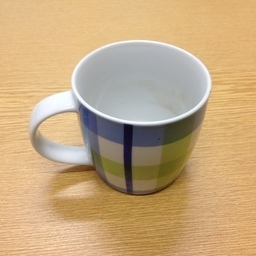
\includegraphics[width=.12\linewidth]{object3} & Yes & No & No & No & Yes & No \\ 
4 & 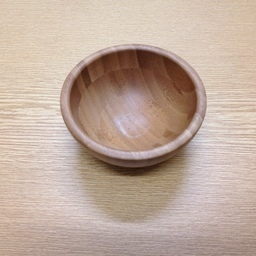
\includegraphics[width=.12\linewidth]{object4} & No & No & No & No & No & No \\ 
5 & \includegraphics[width=.12\linewidth]{object5} & No & No & No & No & No & No \\ 
6 & \includegraphics[width=.12\linewidth]{object6} & Yes & No & No & No & Yes & No \\ 
7 & \includegraphics[width=.12\linewidth]{object7} & No & No & No & No & Yes & No \\ 
8 & \includegraphics[width=.12\linewidth]{object9} & No & No & No & Yes & No & No \\ 
9 & \includegraphics[width=.12\linewidth]{object10} & No & No & No & Yes & No & No \\ 
10 & \includegraphics[width=.12\linewidth]{object11} & No & No & No & Yes & No & No \\ 
11 & \includegraphics[width=.12\linewidth]{object12} & No & No & No & Yes & No & No \\ 
12 & 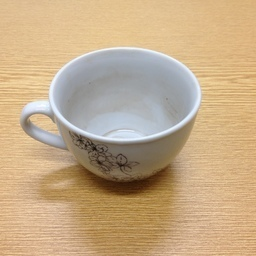
\includegraphics[width=.12\linewidth]{object13} & No & No & No & No & Yes & No \\ 
13 & \includegraphics[width=.12\linewidth]{object14} & No & No & No & Yes & No & No \\ 
14 & 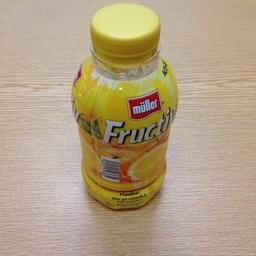
\includegraphics[width=.12\linewidth]{object16} & No & Yes & Yes & No & No & No \\ 
15 & \includegraphics[width=.12\linewidth]{object17} & No & No & Yes & No & No & Yes \\ 
16 & \includegraphics[width=.12\linewidth]{object18} & No & No & No & No & No & No \\ 
17 & 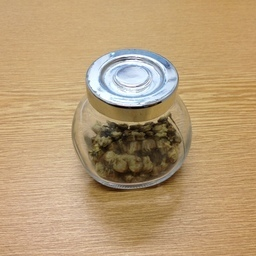
\includegraphics[width=.12\linewidth]{object19} & No & Yes & No & No & Yes & Yes \\ 
18 & 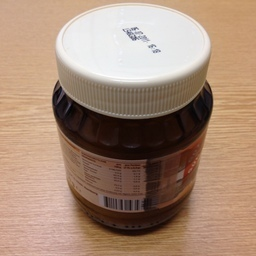
\includegraphics[width=.12\linewidth]{object20} & No & Yes & No & No & Yes & No \\ 
19 & \includegraphics[width=.12\linewidth]{object21} & No & Yes & No & No & Yes & No \\ 
20 & \includegraphics[width=.12\linewidth]{object22} & No & Yes & No & No & Yes & No \\ 
21 & \includegraphics[width=.12\linewidth]{object23} & Yes & No & No & No & Yes & No \\ 
22 & 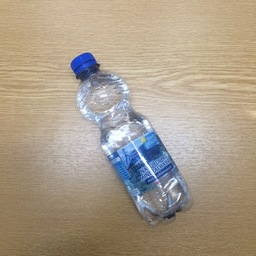
\includegraphics[width=.12\linewidth]{object24} & No & Yes & Yes & No & No & Yes \\ 
23 & \includegraphics[width=.12\linewidth]{object25} & No & No & No & No & Yes & No \\ 
24 & \includegraphics[width=.12\linewidth]{object26} & No & No & No & No & No & Yes \\ 
25 & \includegraphics[width=.12\linewidth]{object27} & No & No & No & No & Yes & No \\ 
26 & \includegraphics[width=.12\linewidth]{object28} & No & No & No & No & No & No \\ 
27 & \includegraphics[width=.12\linewidth]{object29} & No & No & Yes & No & No & Yes \\ 
28 & 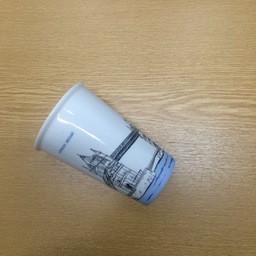
\includegraphics[width=.12\linewidth]{object30} & Yes & No & No & No & Yes & No \\ 
29 & 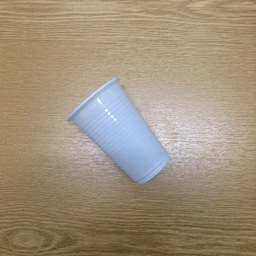
\includegraphics[width=.12\linewidth]{object31} & No & No & Yes & No & No & No \\ 
30 & \includegraphics[width=.12\linewidth]{object32} & No & Yes & No & No & Yes & No \\ 
31 & \includegraphics[width=.12\linewidth]{object33} & No & No & Yes & No & No & No \\ 
32 & \includegraphics[width=.12\linewidth]{object34} & No & No & Yes & No & No & No \\ 
33 & \includegraphics[width=.12\linewidth]{object35} & No & No & Yes & No & No & Yes \\ 
\end{longtable}

\cleardoublepage

% ... add as much appendices as you need (one can also add source code, for example)

%\chapter{}

\fancyhead[LE,RO]{\it Bibliography}          % A bibliography never have a letter or numbering!
\bibliographystyle{abbrv}                    % Style for presenting the literature
\addcontentsline{toc}{chapter}{Bibliography} % Add to the TOC
\bibliography{thesis}
\cleardoublepage

%%%%%%%%%%%%%%%%%%%%%%%%%%%%
% Formal page 1
\vspace{2cm}
\chapter*{Erkl\"arung der Urheberschaft}
\fancyhead[LE]{\it Erkl\"arung der Urheberschaft}
Ich versichere an Eides statt, dass ich die \trtype{} im Studiengang \trcourseofstudies{} selbstst\"andig verfasst und keine anderen als die angegebenen Hilfsmittel -- insbesondere keine im Quellenverzeichnis nicht benannten Internet-Quellen -- benutzt habe. Alle Stellen, die w\"ortlich oder sinngem\"a{\ss} aus Ver\"offentlichungen entnommen wurden, sind als solche kenntlich gemacht. Ich versichere weiterhin, dass ich die Arbeit vorher nicht in einem anderen Pr\"ufungsverfahren eingereicht habe und die eingereichte schriftliche Fassung der auf dem elektronischen Speichermedium entspricht.

\vspace{4cm}
\noindent Ort, Datum \hfill Unterschrift

%The backcover is always empty
\newpage
\thispagestyle{empty}
\hspace{1cm}
\newpage

%%%%%%%%%%%%%%%%%%%%%%%%%%%%
% Formal page 2
\vspace{2cm}
\chapter*{Erkl\"arung zur Ver\"offentlichung}
\fancyhead[LE]{\it Erkl\"arung der Ver\"offentlichung}
Ich erkl\"are mein Einverst\"andnis mit der Einstellung dieser \trtype{} in den Bestand der Bibliothek.

\vspace{4cm}
\noindent Ort, Datum \hfill Unterschrift

%The backcover is always empty
\newpage
\thispagestyle{empty}
\hspace{1cm}
\newpage

\end{document}

